\pdfminorversion=4
\documentclass[aspectratio=169]{beamer}

\mode<presentation>
{
  \usetheme{default}
  \usecolortheme{default}
  \usefonttheme{default}
  \setbeamertemplate{navigation symbols}{}
  \setbeamertemplate{caption}[numbered]
  \setbeamertemplate{footline}[frame number]  % or "page number"
  \setbeamercolor{frametitle}{fg=white}
  \setbeamercolor{footline}{fg=black}
} 

\usepackage[english]{babel}
\usepackage[utf8x]{inputenc}
\usepackage{tikz}
\usepackage{courier}
\usepackage{array}
\usepackage{bold-extra}
\usepackage{minted}
\usepackage[thicklines]{cancel}
\usepackage{fancyvrb}

\xdefinecolor{dianablue}{rgb}{0.18,0.24,0.31}
\xdefinecolor{darkblue}{rgb}{0.1,0.1,0.7}
\xdefinecolor{darkgreen}{rgb}{0,0.5,0}
\xdefinecolor{darkgrey}{rgb}{0.35,0.35,0.35}
\xdefinecolor{darkorange}{rgb}{0.8,0.5,0}
\xdefinecolor{darkred}{rgb}{0.7,0,0}
\definecolor{darkgreen}{rgb}{0,0.6,0}
\definecolor{mauve}{rgb}{0.58,0,0.82}

\title[2021-05-21-dasksummit-awkward-collection]{An Awkward Dask Collection}
\author{Jim Pivarski}
\institute{Princeton University -- IRIS-HEP}
\date{May 21, 2021}

\usetikzlibrary{shapes.callouts}

\begin{document}

\logo{\pgfputat{\pgfxy(0.11, 7.4)}{\pgfbox[right,base]{\tikz{\filldraw[fill=dianablue, draw=none] (0 cm, 0 cm) rectangle (50 cm, 1 cm);}\mbox{\hspace{-8 cm}
\includegraphics[height=1 cm]{princeton-logo-long.png}\hspace{0.1 cm}\raisebox{0.1 cm}{
\includegraphics[height=0.8 cm]{iris-hep-logo-long.png}}\hspace{0.1 cm}}}}}

\begin{frame}
  \titlepage
\end{frame}

\logo{\pgfputat{\pgfxy(0.11, 7.4)}{\pgfbox[right,base]{\tikz{\filldraw[fill=dianablue, draw=none] (0 cm, 0 cm) rectangle (50 cm, 1 cm);}\mbox{\hspace{-8 cm}
\includegraphics[height=1 cm]{princeton-logo.png}\hspace{0.1 cm}\raisebox{0.1 cm}{
\includegraphics[height=0.8 cm]{iris-hep-logo.png}}\hspace{0.1 cm}}}}}

% Uncomment these lines for an automatically generated outline.
%\begin{frame}{Outline}
%  \tableofcontents
%\end{frame}

% START START START START START START START START START START START START START

\begin{frame}{Dask collection types}
\large

\vspace{0.5 cm}
Dask has three built-in collection types: $\underbrace{\mbox{\textcolor{darkblue}{array},}}_{\mbox{NumPy}}$ $\underbrace{\mbox{\textcolor{darkblue}{dataframe\vphantom{y}},}}_{\mbox{Pandas}}$ and $\underbrace{\mbox{\textcolor{darkblue}{bag\vphantom{y}}.}}_{\mbox{Python}}$

\vspace{1 cm}
\uncover<2->{As well as hidden collection type(s): \textcolor{darkblue}{xarray} (and others?), using Dask internally.}
\end{frame}

\begin{frame}[fragile]{Awkward Array generalizes NumPy}
\small
\begin{columns}
\column{1.05\linewidth}
\begin{minted}{python}
>>> a = ak.Array([[0, 1, 2], [], [3, 4], [5], [6, 7, 8, 9]])
\end{minted}
\vspace{-0.3 cm}
\begin{uncoverenv}<2->
\begin{minted}{python}
>>> a[:, 1:]
<Array [[1, 2], [], [4], [], [7, 8, 9]] type='5 * var * int64'>
\end{minted}
\end{uncoverenv}
\vspace{-0.3 cm}
\begin{uncoverenv}<3->
\begin{minted}{python}
>>> b = ak.Array([
...     {"z": 1.1}, {"z": 2.2}, {"z": 3.3}, {"z": 4.4}, {"z": 5.5}
... ])
\end{minted}
\end{uncoverenv}
\vspace{-0.3 cm}
\begin{uncoverenv}<4->
\begin{minted}{python}
>>> b["z"]
<Array [1.1, 2.2, 3.3, 4.4, 5.5] type='5 * float64'>
\end{minted}
\end{uncoverenv}
\vspace{-0.3 cm}
\begin{uncoverenv}<5->
\begin{minted}{python}
>>> c = ak.zip({"x": a, "y": b}); c
<Array [[{x: 0, y: {z: 1.1}, ... y: {z: 5.5}}]] type='5 * var * {...'>
\end{minted}
\end{uncoverenv}
\vspace{-0.3 cm}
\begin{uncoverenv}<6->
\begin{minted}{python}
>>> np.sqrt(c.y.z)
<Array [[1.05, 1.05, 1.05, ... 2.35, 2.35]] type='5 * var * float64'>
\end{minted}
\end{uncoverenv}
\vspace{-0.3 cm}
\begin{uncoverenv}<7->
\begin{minted}{python}
>>> np.sum(c.y.z, axis=0)
<Array [14.3, 9.9, 6.6, 5.5] type='4 * float64'>
\end{minted}
\end{uncoverenv}
\vspace{-0.3 cm}
\begin{uncoverenv}<8->
\begin{minted}{python}
>>> np.sum(c.y.z, axis=1)
<Array [3.3, 0, 6.6, 4.4, 22] type='5 * float64'>
\end{minted}
\end{uncoverenv}
\end{columns}
\end{frame}

\begin{frame}[fragile]{Including functions that have no equivalent in NumPy}
\small
\vspace{-0.75 cm}
\begin{columns}
\column{1.05\linewidth}
\begin{minted}{python}
>>> a = ak.Array([[0, 1, 2], [], [3, 4]])
>>> b = ak.Array([["one", "two"], ["one"], ["one"]])
>>> ak.cartesian({"a": a, "b": b}, axis=1).tolist()
[
    [
        {'a': 0, 'b': 'one'},
        {'a': 0, 'b': 'two'},
        {'a': 1, 'b': 'one'},
        {'a': 1, 'b': 'two'},
        {'a': 2, 'b': 'one'},
        {'a': 2, 'b': 'two'},
    ],
    [],
    [
        {'a': 3, 'b': 'one'},
        {'a': 4, 'b': 'one'},
    ],
]
\end{minted}

\vspace{-5.5 cm}
\hfill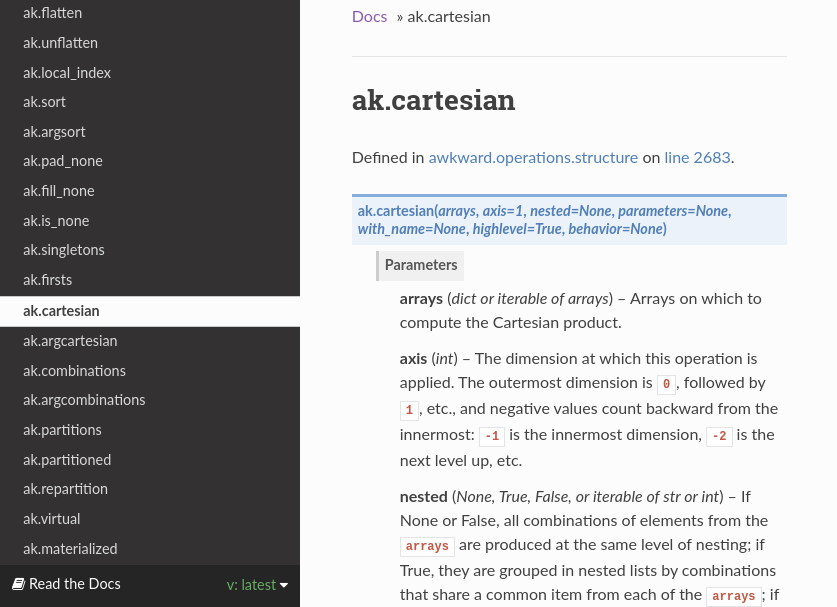
\includegraphics[height=4 cm]{docs-cartesian.png}
\end{columns}
\end{frame}

\begin{frame}{Awkward Arrays as Dask arrays?}
\Large
It might seem like we could use \mintinline{python}{dask.array} for Awkward Arrays,

but\ldots

\large
\vspace{0.5 cm}
\begin{itemize}\setlength{\itemsep}{0.5 cm}
\item<2-> Awkward Arrays do not have \mintinline{python}{shape} and \mintinline{python}{dtype}, and you quickly run into Dask operations that expect them to.
\item<3-> Dask doesn't know that \mintinline{python}{ak.*} are fundamental operations (DAG nodes), just as \mintinline{python}{np.*} are.
\item<4-> \href{https://github.com/scikit-hep/uproot3}{\textcolor{blue}{\underline{scikit-hep/uproot3}}}'s git history is littered with attempts to make it work.
\end{itemize}
\end{frame}

\begin{frame}{What about bags or dataframes?}
\begin{columns}
\column{0.47\linewidth}
\vspace{0.25 cm}
\only<1>{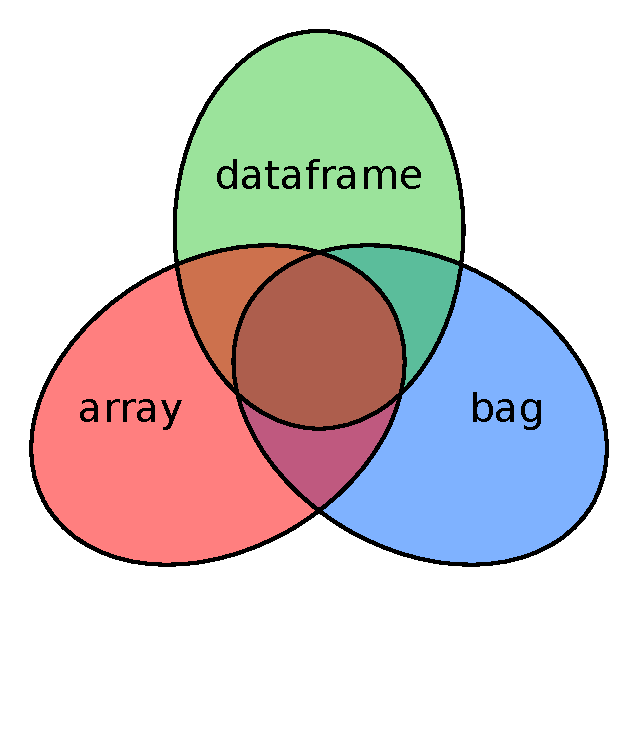
\includegraphics[width=\linewidth]{venn-array-bag-dataframe-1.pdf}}\only<2->{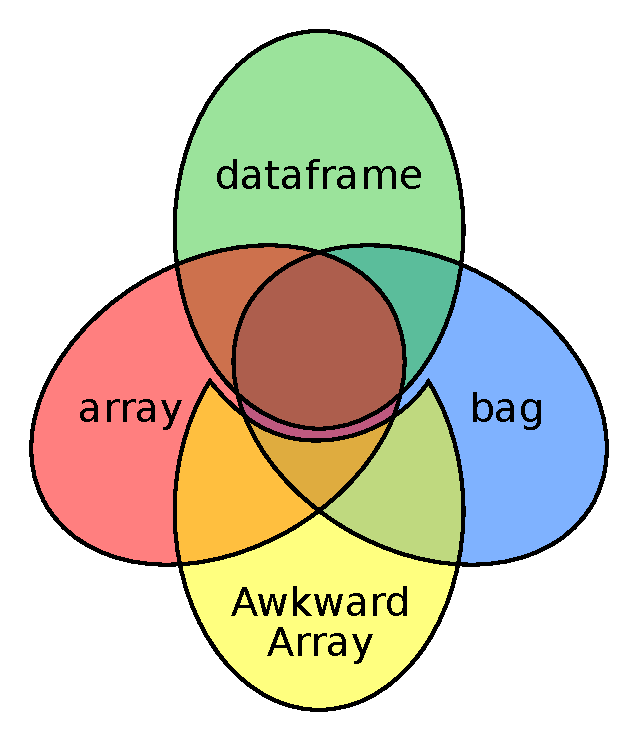
\includegraphics[width=\linewidth]{venn-array-bag-dataframe-2.pdf}}

\column{0.55\linewidth}
\uncover<3->{\textcolor{darkblue}{Like array:} in that the elements have a single type, rich slicing semantics, and compiled loops.}

\vspace{0.25 cm}
\uncover<3->{\textcolor{darkblue}{Unlike array:} in that the type can be nested, variable-length, nullable, and heterogeneous unions, partitioning only makes sense in 1D, includes fundamental functions beyond NumPy.}

\vspace{0.25 cm}
\uncover<4->{\textcolor{darkblue}{Like bag:} in type generality and 1D partitioning.}

\vspace{0.25 cm}
\uncover<4->{\textcolor{darkblue}{Unlike bag:} in having a single type, rich slicing, an \mintinline{python}{axis} concept, and compiled loops.}

\vspace{0.25 cm}
\uncover<5->{\textcolor{darkblue}{Unlike dataframe:} in not having an index and not having columns, apart from record fields.}

\vspace{0.25 cm}
\uncover<6->{\textcolor{darkorange}{\bf Somewhere between an array and a bag.}}
\end{columns}
\end{frame}

\begin{frame}{Fundamental question}
\Large

{\it If} Awkward Arrays are to be integrated with Dask, {\it then} they need to be a new collection type.

\vspace{1 cm}
\uncover<2->{\textcolor{darkblue}{But do we really need Awkward Dask arrays?}}
\end{frame}

\begin{frame}{Specifically, for particle physics}
\Large

\textcolor{darkblue}{Do physicists need out-of-core datasets?} \uncover<2->{\textcolor{darkorange}{\bf Yes!}}

\uncover<2->{\phantom{Do physicists need out-of-core datasets?} typical RAM = 10~GB}

\uncover<2->{\phantom{Do physicists need out-of-core datasets?} typical analysis = 10~TB}

\vspace{1 cm}

\uncover<3->{\textcolor{darkblue}{Do physicists need a distributed array abstraction?}} \uncover<4->{\textcolor{darkorange}{\bf Arguably.}}
\end{frame}

\begin{frame}[fragile]{LHC analyses can be neatly divided into map-reduce}
\vspace{0.25 cm}
\small
\begin{minted}{python}
import coffea

class MyAnalysis(coffea.processor.ProcessorABC):
    def __init__(self, **parameters):
        self.parameters = parameters
        self.accumulator = ... # histograms

    def process(self, df):
        output = self.accumulator.identity()
        # analyze one partition of data, filling histograms...
        return output

    def postprocess(self, accumulator):
        # final touches on combined histograms, like scaling...
        return accumulator

analysis = MyAnalysis(parameter1=...)  # run with a Dask scheduler
\end{minted}
\end{frame}

\begin{frame}[fragile]{Moreover, Awkward Array already has a delayed abstraction}
\small
\begin{columns}
\column{1.05\linewidth}
\begin{minted}{python}
>>> def read(i):
...     print("reading", i)
...     return ak.Array(range(10))
... 
>>> form = ak.forms.Form.from_numpy(np.dtype(np.int64))
>>> array = ak.partitioned([
...     ak.virtual(read, (i,), form=form, length=10) for i in range(5)
... ])
\end{minted}
\vspace{-0.3 cm}
\begin{uncoverenv}<2->
\begin{minted}{python}
>>> array[:5]
reading 0
<Array [0, 1, 2, 3, 4] type='5 * int64'>
\end{minted}
\end{uncoverenv}
\begin{uncoverenv}<3->
\vspace{-0.3 cm}
\begin{minted}{python}
>>> array[:15]
reading 1
<Array [0, 1, 2, 3, 4, 5, ... 9, 0, 1, 2, 3, 4] type='15 * int64'>
\end{minted}
\end{uncoverenv}
\vspace{-0.3 cm}
\begin{uncoverenv}<4->
\begin{minted}{python}
>>> array
reading 4
<Array [0, 1, 2, 3, 4, 5, ... 4, 5, 6, 7, 8, 9] type='50 * int64'>
\end{minted}
\end{uncoverenv}
\end{columns}
\end{frame}

\begin{frame}[fragile]{Moreover, Awkward Array already has a delayed abstraction}
\small
\begin{columns}
\column{1.05\linewidth}
\begin{minted}{python}
>>> array.layout
\end{minted}
\vspace{-0.4 cm}
\begin{Verbatim}[commandchars=\\\{\}]
<\textcolor{darkgreen}{\textbf{IrregularlyPartitionedArray}}>
    <\textcolor{darkgreen}{\textbf{partition}} start="0" stop="10">
        <\textcolor{blue}{\textbf{VirtualArray}} cache_key="ak0">
            <ArrayGenerator f="<function read at 0x7f...>" args="(0,)">
                <length>10</length>
                <form>\{
                    "class": "NumpyArray",
                    "itemsize": 8,
                    "format": "l",
                    "primitive": "int64"
                \}</form>
            </ArrayGenerator>
            <ArrayCache mapping="\{\}"/>
        </\textcolor{blue}{\textbf{VirtualArray}}>
    </\textcolor{darkgreen}{\textbf{partition}}>
    <\textcolor{darkgreen}{\textbf{partition}} start="10" stop="20">
        ...
\end{Verbatim}
\end{columns}
\end{frame}




\end{document}
